\section{Free Trade}
\paragraph{This question can be treated as a variation of the birthday paradox, The trader in \( n^{th} \) place gets the free trade if all the traders in front of him have unique ID numbers and he has an ID number equal to one of them. \\\\This is given by: \\\\}
$\text{Probablity that first n-1 traders have unique IDs} = \prod_{i=0}^{n-2} (\frac{200-i}{200})$\\\\
$\text{Probablity that $n^{th}$ trader has matching ID with someone in front} = (\frac{n-1}{200})$
\begin{align*}
	P(\text{\(1^{st}\) trader gets the free trade}) & = 0                                                           \\\\
	P(\text{\(2^{nd}\) trader gets the free trade}) & = \frac{200}{200} \times \frac{1}{200}                        \\\\
	P(\text{\(3^{rd}\) trader gets the free trade}) & = \frac{200}{200} \times \frac{199}{200} \times \frac{2}{200} \\
\end{align*}
This can be generalised for the \(n^{th}\) trader (\(n \leq 200\)) as follows
\begin{align*}
	P(\text{\(n^{th}\) trader gets the free trade}) = \frac{\prod_{i=0}^{n-2} (200-i) \times (n-1)}{200^n}
\end{align*}
\begin{align*}
	P(n^{th} \text{ trader getting the free trade}) = P((n-1)^{th} \text{ trader getting the free trade}) \times \frac{202-n}{200} \times \frac{n-1}{n-2}
\end{align*}
\begin{align*}
	\frac{202-n}{200} \times \frac{n-1}{n-2} \geq 1 \text{ } \forall n \leq 15 \\
	\frac{202-n}{200} \times \frac{n-1}{n-2} \leq 1 \text{ } \forall n \geq 16
\end{align*}
$\therefore$ P($n^{th}$ trader getting the free trade) will be maximum for $n = 15$\\
We can verify this by writing a python program to find these values and plot them\\
\begin{lstlisting}[language=Python, caption={Python code to calculate the probability}]
import matplotlib.pyplot as plt

placelist = []
probablitylist = []
maxplace,maxprobablity = 0,0

plt.figure(dpi=600)
for x in range(1,100):
    probablity = 1
    for i in range(x-1):
        probablity *= ((200-i)/200)
    probablity*=(x-1)/200
    placelist.append(x)
    probablitylist.append(probablity)
    if(probablity>maxprobablity):
        maxprobablity = probablity
        maxplace = x
    print(f"{x} th place: {probablity}")

plt.scatter(placelist,probablitylist)
plt.axvline(maxplace)
plt.xticks([maxplace])
plt.axhline(maxprobablity)
plt.yticks([maxprobablity])
plt.xlabel("Place ")
plt.ylabel("Probablity of getting the free trade")
print(f"Max value is {maxprobablity} for place = {maxplace}")

plt.savefig("./Q5GraphPlot.png",bbox_inches='tight')
\end{lstlisting}

% \vspace{lcm}

The above code results in the following graph:
\begin{figure}[h]
	\centering
	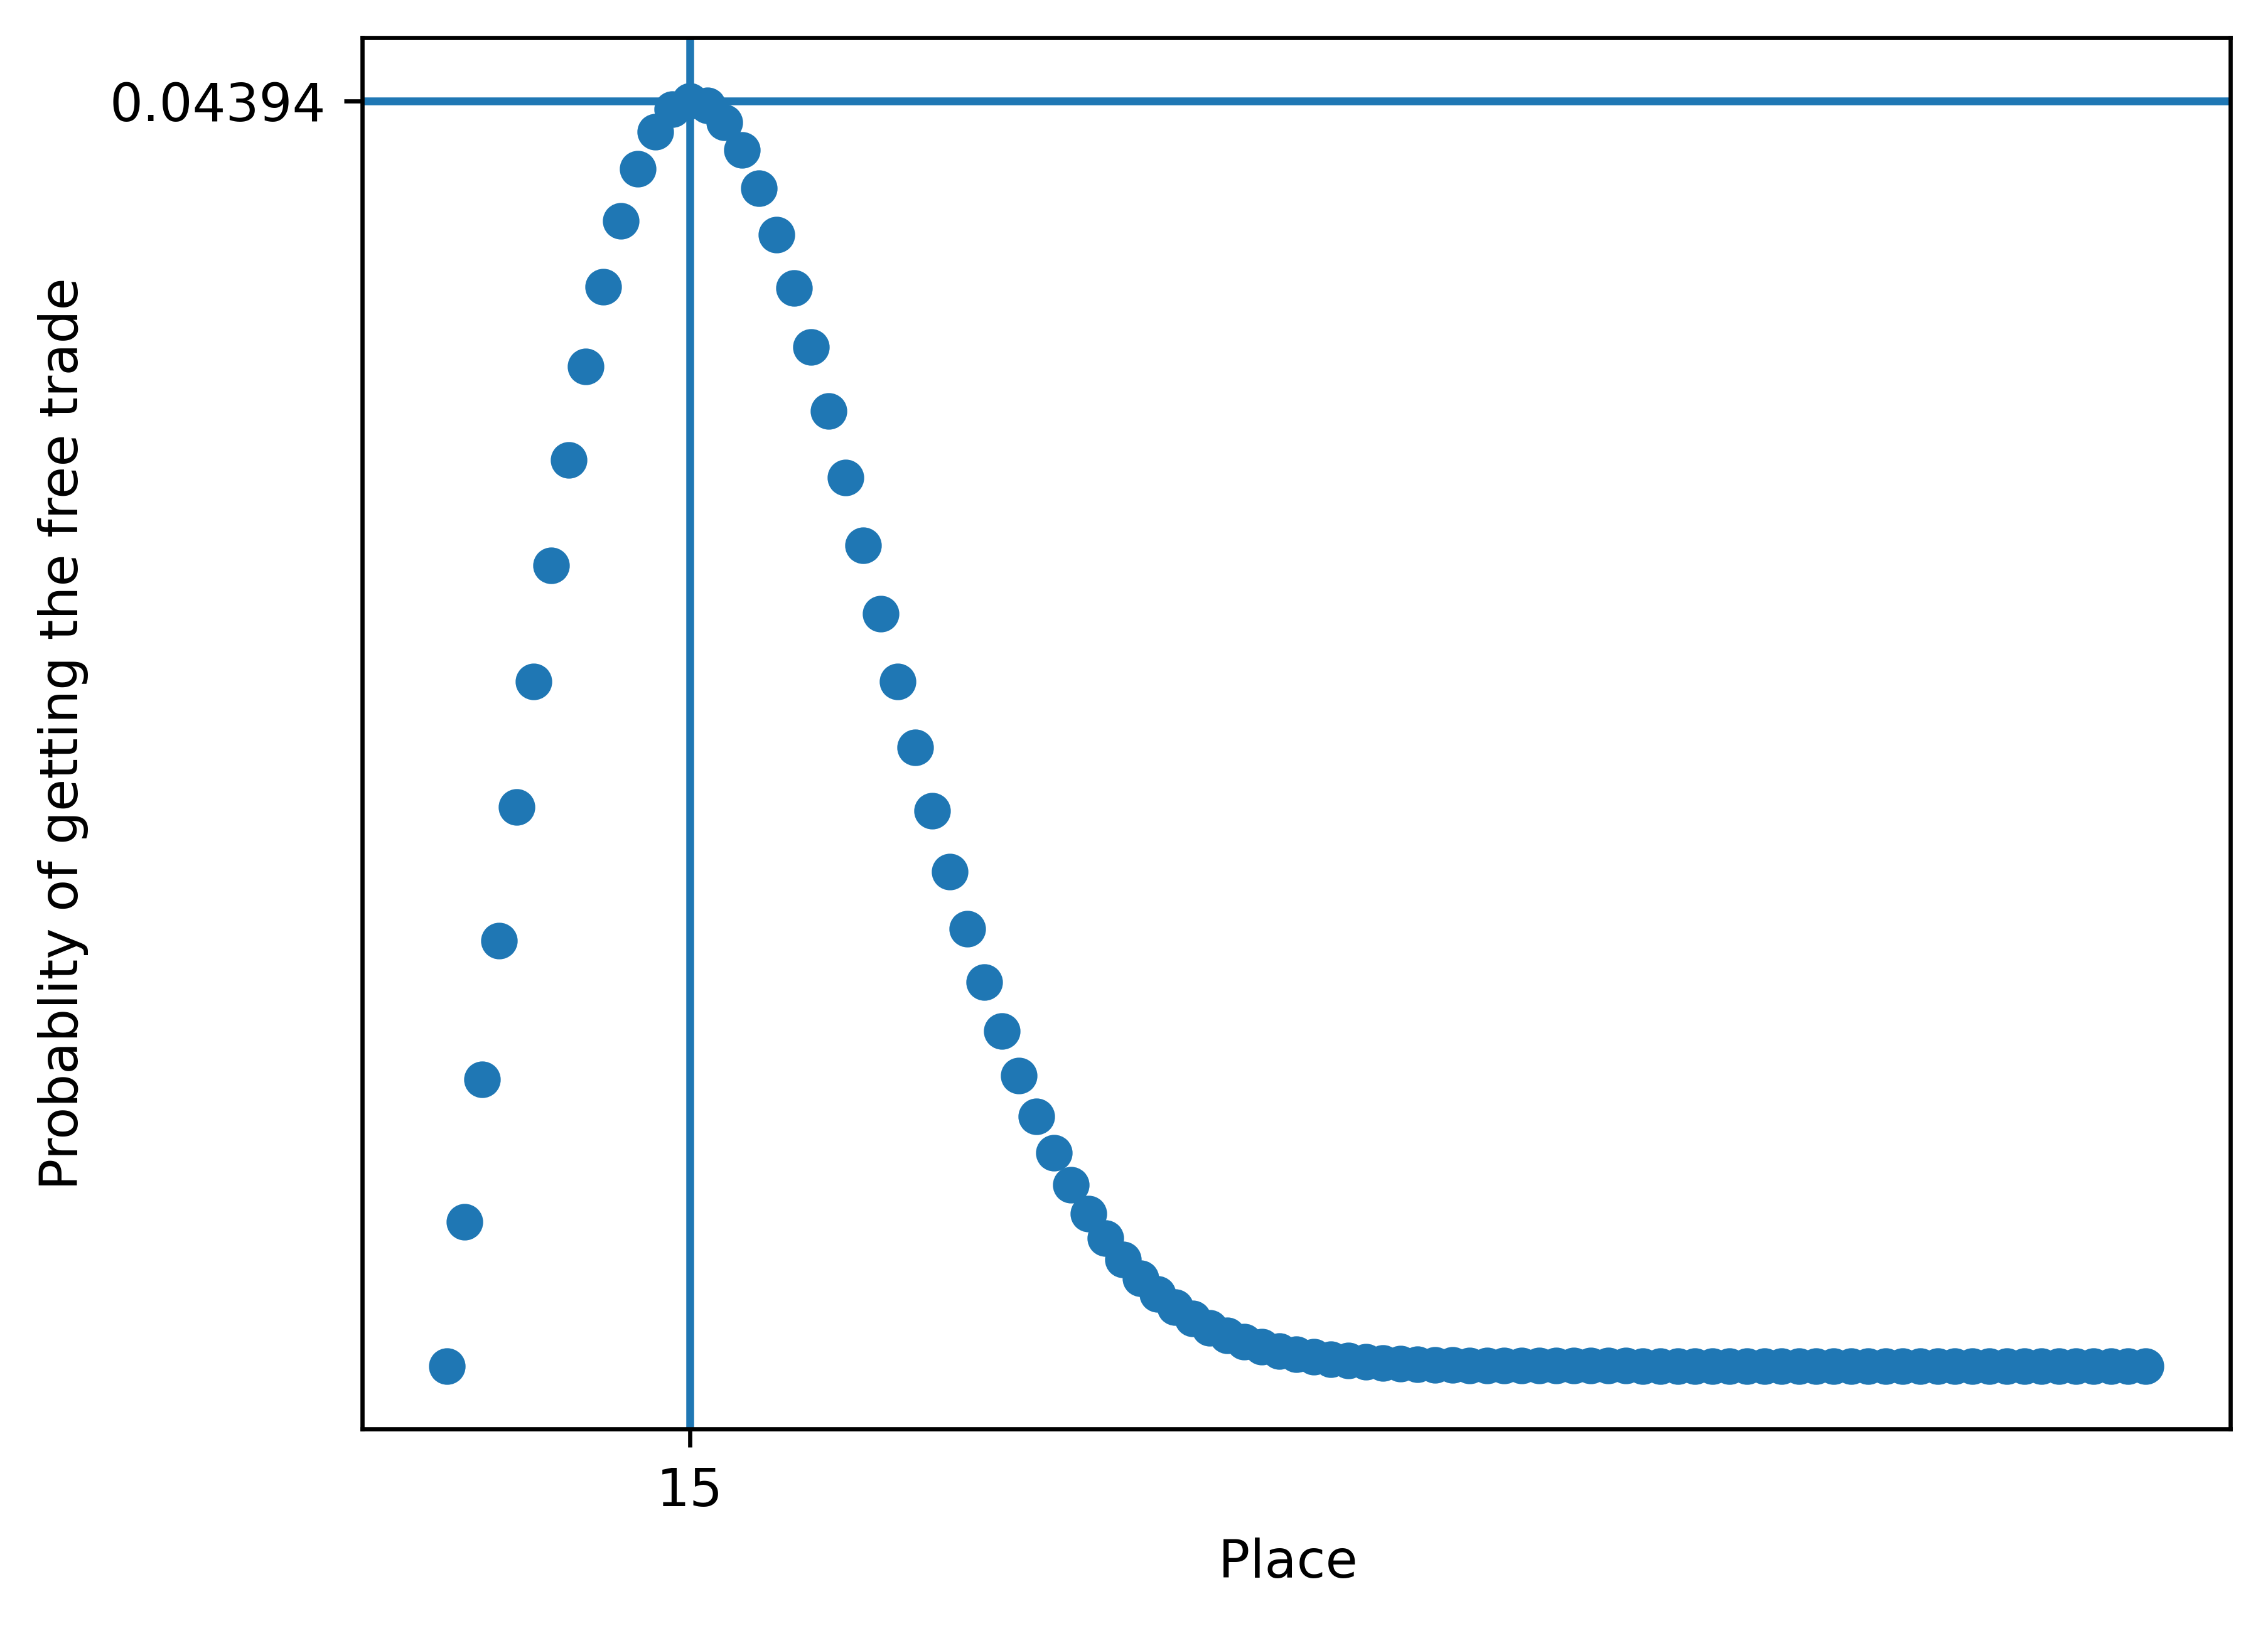
\includegraphics[width=0.8\textwidth]{img/Q5 Graph Plot.png}
	\caption{Graph of the probability of getting the free trade}
\end{figure}

\paragraph{$\therefore$ We should position ourselves at the \(15^{th}\) place to maximize the probability of getting the free trade.}
